\subsection{Results for Random Dictionaries \label{sec:random-results}}

\begin{figure}
	\begin{center}
	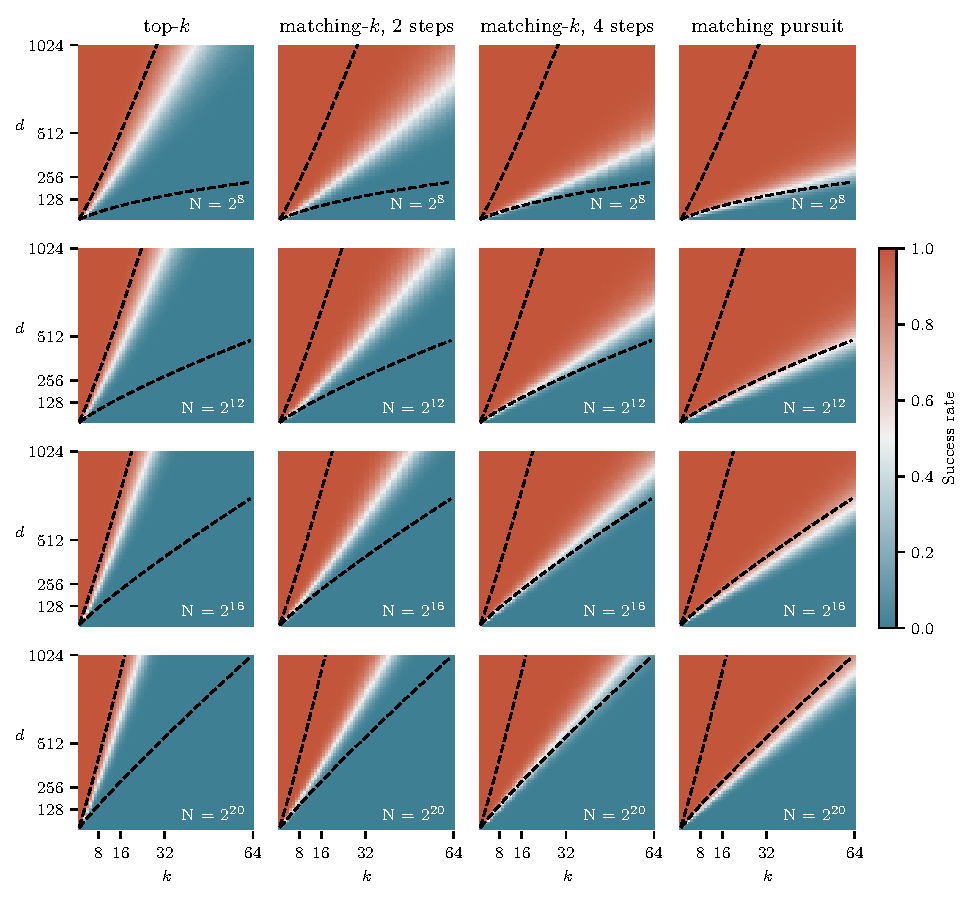
\includegraphics[width=\textwidth]{../figures/pursuit}
	\caption{Empirical performance of a variety of different decoding methods at reading a $k$-element subset of $[N]$ from a $d$-dimensional superposition code with a Rademacher dictionary.}
	\label{fig:pursuit}
	\end{center}
\end{figure}

\begin{figure}
	\begin{center}
	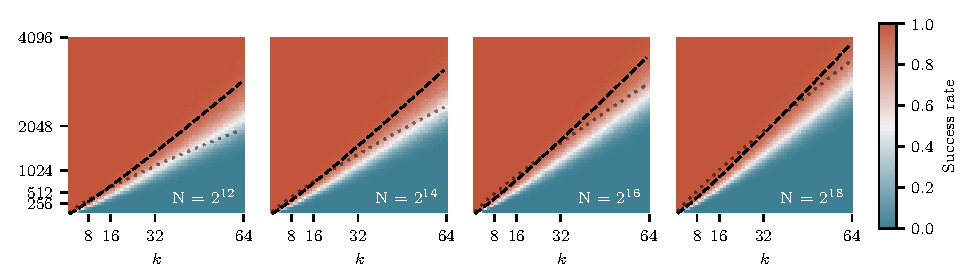
\includegraphics[width=\textwidth]{../figures/top_k}
	\caption{The prediciton of Proposition \Cref{prop:sufficient-cond} agrees well with numerical experiments.}
	\label{fig:top-k}
	\end{center}
\end{figure}

\begin{figure}
	\begin{center}
	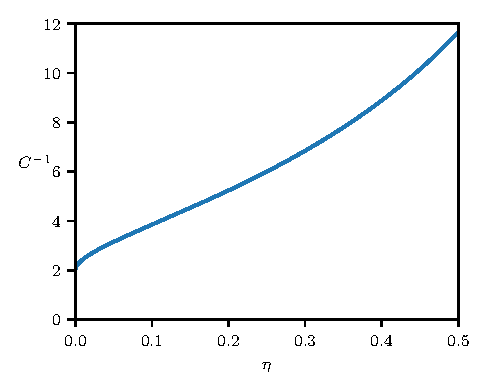
\includegraphics[width=0.5 \textwidth]{../figures/capacity}
	\caption{Inverse channel capacity (in nats per dimension) predicted by \Cref{prop:sufficient-cond}.}
	\label{fig:capacity}
	\end{center}
\end{figure}

Our first result on random dictionaries provides an

\begin{proposition} \label{prop:necessary-cond}
    Let $F$ and $G$ be as above, and let $C < 2.$ Then for sufficiently large $N,$ $\Pp(G(F(Y)) = Y) < 1/2.$
\end{proposition}

This shows that

\begin{proposition} \label{prop:sufficient-cond}
	For $\epsilon \in (0, 1),$ let $\ln k \le \epsilon \ln N,$ and let
	$$
	\kappa > 2 + 4 \sqrt \epsilon + 2 \epsilon.
	$$
	Suppose $d \ge \kappa \ln N.$ Then for sufficiently large $N,$ $G(F(Y)) = Y$ with arbitrarily high probability.
\end{proposition}

Since
$$
2 + 4 \sqrt \epsilon + 2 \epsilon \le 4(1  + \epsilon)
$$
and when $k = N^\epsilon,$ $4(1 + \epsilon) k \ln N = 4 k \ln (N / k),$ \Cref{prop:sufficient-cond} shows that.

This predictions agrees well with numerical experiments, graphed in \Cref{fig:one-step}. In fact, even as $N$ varies over several orders of magnitude, the slightly weaker condition $d \ge 8 k \ln N$ characterizes the regime where the set $Y$ can be decoded with reasonably high probability by threshold decoding.

Top-$k$ decoding performs significantly better but admits a similar ``rule of thumb'': for all values of $N$ trialed, $d = 4 k \ln k N$ is very close to the smallest dimension needed for top-$k$ decoding to succeed with high probability. See \Cref{appendix:top_k} for an informal derivation of this bound.

There are several ways to interpret this conclusion. On one hand, it means that one-step estimates are asymptotically ``inefficient'' in terms of required bitrate when $k$ is moderately large compared to $N.$ More specifically, in a regime where $N$ goes to infinity but $\ln k / \ln N$ converges to $1,$ we predict that one-step estimates require the ratio $d/H$ to diverge to infinity.

In particular, one-step estimates are asymptotically inefficient when $k/N \ge \epsilon$ for some positive $\epsilon.$ Indeed, to have $d \ge 4 k \ln N$ in this case we would need $d = \Omega(N \ln(N)),$ while the entropy of $Y$ is only $O(N).$ In contrast, a hallmark result of compressive sensing implies that, when $k/N \le \epsilon,$ the vector $y$ can be recovered from its image $F y$ under a random projection by a certain \textit{convex} optimization problem so long as $d \ge \kappa(\epsilon) N$ for some constant $\kappa(\epsilon)$; for example, see \cite{candes_decoding_2005}. The failure of our one-step estimates in this particular regime is easy to prove.

On the other hand, in a sparser regime where $\ln k / \ln N < \epsilon$ for some $\epsilon < 1,$ it follows from our analysis that one-step estimates are ``information-efficient'' in the sense that they can be decoded from superposition codes that achieve bitrates $H/d$ larger than some positive $\delta.$ However, it is also of interest to have \textit{non-asymptotic} information on the required bitrate. From \Cref{eq:bitrate} we find that one-step estimates need at least $4 \ln 2 \approx 2.8$ bits per dimension even for small $k.$ When $k = 2^8$ and $N = 2^{20}$ this number rises to about $4.1,$ and the experiments of \Cref{fig:one-step} show that this factor is in fact slightly optimistic. If we use threshold decoding instead of top-$k,$ we need $8$ dimensions per bit! Can other inference algorithms do significantly better?

There is an extensive literature on theory of compressive sensing. \cite{reeves_all-or-nothing_2019} shows that, in our language, superposition codes with a random dictionary are essentially optimal in the information-theoretic sense when ideal maximum-likelihood inference is used as the decoder. A series of earlier works (\cite{joseph_least_2012, joseph_fast_2014, rush_capacity-achieving_2017}) on superposition codes also showed that, under some special conditions on $y$, certain decoding schemes admit bitrates up to theoretical channel capacity in the presence of Gaussian noise. However, to our knowledge, practical guarantees on the performance of iterative methods are not available for our range of $k$ and $N.$

\Cref{fig:mp} shows the results of a numerical experiment using an iterative method called \textit{matching pursuit}, first suggested in \cite{bergeaud_matching_1995}. This is a simple ``greedy'' algorithm that initializes $y = 0$ and, at each of $k$ iterations, increments the index of $y$ whose corresponding codeword has largest inner product with $x - Fy.$

Matching pursuit far outperforms top-$k$ decoding for the range of $N$ and $k$ considered earlier. When $d \ge 1.3 \log_2 (e N /k)$ and $N > 2^{16},$ our experiments show that matching pursuit is very reliable. In other words, matching pursuit can reliably infer a sparse vector from just $1.3$ dimensions per bit. In \Cref{appendix:bp} we find that a more computationally expensive algorithm called basis pursuit can do slightly better, requiring only 0.8 dimensions per bit.
